\documentclass[a4paper,11pt]{article}
\usepackage[british]{babel}
\usepackage{fullpage}
\usepackage{amsmath,amssymb}
\usepackage{multirow}
\usepackage{caption}
\usepackage{tikz,pgfplots}
\usepackage{hyperref}
\usepackage{graphicx}
\usepackage{enumitem}
\title{\textbf{Low-level Parallel Programming (course 1DL550) \\
    Uppsala University -- Spring 2015 \\
    Report for Lab 2 by Team 14}}
\author{Fredrik Larsson \and Jimmy Holm \and Per Bergqwist}
\date{\today}
\begin{document}
\maketitle
\section{System specification}
The CPU of the system used for gathering the data presented was an
Intel i7 2600k running at a frequency of 4GHz. The system was able to
use four cores with Hyper-threading enabled, meaning a possibility of
using eight logical cores simultaneously with the drawback that the
performance gain from using more than four cores varies depending on
the tasks. To collect the data for OpenCL an AMD HD7970 GPU with 3GB
of memory was used running with the standard clock of 925MHz.
\section{Plot}
\subsection{scenario.xml}
\begin{center}
  \pgfplotsset{grid style={dotted,gray}}
  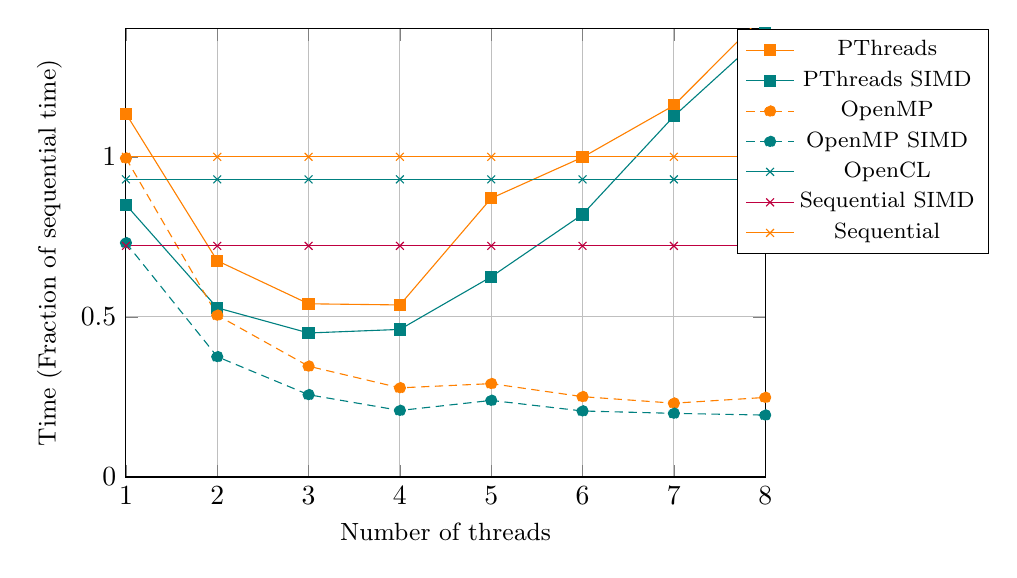
\begin{tikzpicture}
    \begin{axis}[
        width=0.8\textwidth,
        height=0.6\textwidth,
        xtick={1,...,8},
        xmin=1,
        xmax=8,
        ymin=0,
        ymax=1.4,
        grid=both,
        legend style={at={(1.35,1)},anchor=north east},
        legend entries={
          \footnotesize{PThreads},
          \footnotesize{PThreads SIMD},
          \footnotesize{OpenMP},
          \footnotesize{OpenMP SIMD},
          \footnotesize{OpenCL},
          \footnotesize{Sequential SIMD},
          \footnotesize{Sequential}
        },
        xlabel={\small Number of threads},
        ylabel={\small Time (Fraction of sequential time)}
      ]
      %% pthreads
      \addplot[color=orange,mark=square*] coordinates{
        (1,1.13478)
        (2,0.675423)
        (3,0.541)
        (4,0.537409)
        (5,0.870581)
        (6,0.998571)
        (7,1.16046)
        (8,1.44631)
      };
      %% pthreads simd
      \addplot[color=teal,mark=square*] coordinates{
        (1,0.850037)
        (2,0.528359)
        (3,0.449847)
        (4,0.461004)
        (5,0.625313)
        (6,0.820093)
        (7,1.12675)
        (8,1.38598)
      };
      %% omp
      \addplot[densely dashed,color=orange,mark=*] coordinates{
        (1,0.995768)
        (2,0.505261)
        (3,0.3461)
        (4,0.278532)
        (5,0.291689)
        (6,0.250976)
        (7,0.230638)
        (8,0.24856)
      };
      %% omp simd
      \addplot[densely dashed,color=teal,mark=*] coordinates{
        (1,0.731386)
        (2,0.375731)
        (3,0.257043)
        (4,0.207856)
        (5,0.239281)
        (6,0.206265)
        (7,0.198881)
        (8,0.193466)
      };
      %% opencl
      \addplot[color=teal,mark=x] coordinates{
        (1,0.929541)
        (2,0.929541)
        (3,0.929541)
        (4,0.929541)
        (5,0.929541)
        (6,0.929541)
        (7,0.929541)
        (8,0.929541)
      };
      %% simd
      \addplot[color=purple,mark=x] coordinates{
        (1,0.721943)
        (2,0.721943)
        (3,0.721943)
        (4,0.721943)
        (5,0.721943)
        (6,0.721943)
        (7,0.721943)
        (8,0.721943)
      };
      \addplot[color=orange,mark=x] coordinates{
        (1,1)
        (2,1)
        (3,1)
        (4,1)
        (5,1)
        (6,1)
        (7,1)
        (8,1)
      };
      %% \draw (axis cs:2,0.944114) -- (axis cs:14,0.944114);
      %% \draw (axis cs:2,0.722371) -- (axis cs:14,0.722371);
    \end{axis}
  \end{tikzpicture}
\end{center}
\subsection{scenario\_small.xml}
\begin{center}
  \pgfplotsset{grid style={dotted,gray}}
  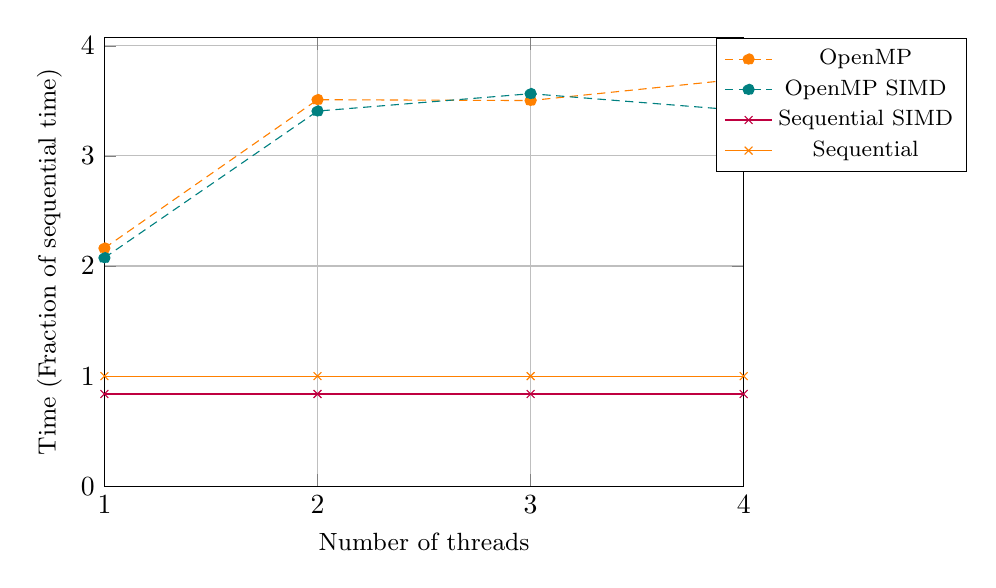
\begin{tikzpicture}
    \begin{axis}[
        width=0.8\textwidth,
        height=0.6\textwidth,
        xtick={1,...,4},
        xmin=1,
        xmax=4,
        ymin=0,
        grid=both,
        legend style={at={(1.35,1)},anchor=north east},
        legend entries={
          \footnotesize{OpenMP},
          \footnotesize{OpenMP SIMD},
          \footnotesize{Sequential SIMD},
          \footnotesize{Sequential}
        },
        xlabel={\small Number of threads},
        ylabel={\small Time (Fraction of sequential time)}
      ]
      %% omp
      \addplot[densely dashed,color=orange,mark=*] coordinates{
        (1,2.1623)
        (2,3.51068)
        (3,3.50279)
        (4,3.7016)
      };
      %% omp simd
      \addplot[densely dashed,color=teal,mark=*] coordinates{
        (1,2.07451)
        (2,3.40727)
        (3,3.56501)
        (4,3.41178)
      };
      %% simd
      \addplot[color=purple,mark=x] coordinates{
        (1,0.837713)
        (2,0.837713)
        (3,0.837713)
        (4,0.837713)
      };
      \addplot[color=orange,mark=x] coordinates{
        (1,1)
        (2,1)
        (3,1)
        (4,1)
      };
    \end{axis}
  \end{tikzpicture}
\end{center}
\section{Questions}
\begin{enumerate}[label=\Alph*.]
\item \textbf{What kind of parallelism is exposed with your code
  refactorization?}\\

\item \textbf{Give a short summary of similarities and differences
  between SIMD and CUDA.}\\

\item \textbf{Which parallelization has been most beneficial in these
  two labs? Support your case using plotted time measurements.}\\

\item \textbf{What kind of code transformations were required for this
  lab, and why were they needed?}\\

\item \textbf{Compare the effort required for each of the four
  parallellization techniques. Would it have made a difference if you
  had to build the program from scratch, instead of using given
  code?}\\

\end{enumerate}
\section{How to run}
The demo runs with a GUI and using the sequential implementation
if no flag has overwritten the settings. The following flags can be
used to alter the demo and change the implementation for the tick
function.
\begin{itemize}[label=,leftmargin=0pt]
\item \textbf{-\--timing-mode} - Without gui.
\item \textbf{-\--pthreads} - Executes the PThreads implementation.
\item \textbf{-\--omp} - Executes the OpenMP implementation.
\item \textbf{-\--opencl} - Executes the OpenCL implementation.
\item \textbf{-\--simd} - Executes the SIMD implementation, can be
  combined with either omp or pthreads.
\item \textbf{-\--threads \textit{number}} - Tells the demo to use
  \textit{number} threads when executing.
\item \textbf{-\--silent} - Does not print to standard output.
\item \textbf{-\--plot} - Stores the timing data to the file
  testdata.txt
\end{itemize}
\end{document}
